\documentclass[12pt]{article}
\usepackage{graphicx}
\usepackage{float}
\usepackage{amsmath}
\title{Experiment 6: ALU}
\author{Annirudh K P\\%
210070009}
\date{September 23, 2022}
\begin{document}

\maketitle

\section{Overview of the experiment}
\paragraph{}
In this experiment, we started working on designs using behavioural modelling on VHDL. The problem statement of this experiment is to design an ALU. The objective of this experiment was to understand the Quartus Design Flow, work with the Xen10 Board, use ScanChain for testbenching, and give us hands on experience over different technical glitches/problems we may face in this piece of software which has been made unwantedly hard.

\section{Experimental Set-up}

\subsection{Design Schematics}
The following design schematics are shown for the ALU 

\begin{figure}[H]
\centering
  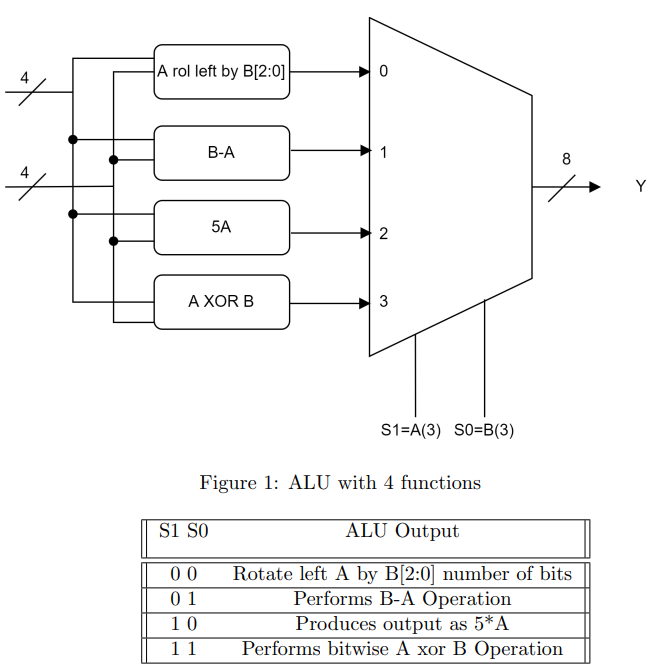
\includegraphics[scale=0.3]{Images/ALU_Design.png}
  \caption{}
\end{figure}

\subsection{Description of Components}
\subsubsection{Multiplier}
\begin{verbatim}
library ieee;
use ieee.std_logic_1164.all;

entity alu_beh is
	generic(
		operand_width : integer:=4);
	port (
		A: in std_logic_vector(operand_width-1 downto 0);
		B: in std_logic_vector(operand_width-1 downto 0);
		op: out std_logic_vector((operand_width*2)-1 downto 0)) ;
end alu_beh;

architecture a1 of alu_beh is
	function sub(A: in std_logic_vector(operand_width-1 downto 0); B: in
	 std_logic_vector(operand_width-1 downto 0))
		return std_logic_vector is
			-- declaring and initializing variables using aggregates
			variable diff : std_logic_vector(operand_width*2-1 downto 0):= (others=>'0');
			variable carry : std_logic:= '1';
			variable borrow: std_logic_vector(3 downto 0);
		begin
			-- Hint: Use for loop to calculate value of "diff" and "carry" variable
			-- Use aggregates to assign values to multiple bits
			L1: for i in 0 to (operand_width-1) loop
				if i=0 then
					diff(i) := A(i) xor B(i);
					borrow(i) := not(A(i)) and B(i);
				else
					diff(i) := A(i) xor B(i) xor borrow(i-1);
					borrow(i) := (not(A(i)) and B(i)) or ((not(A(i) xor B(i))) and borrow(i-1));
				end if;
			end loop L1;
		return diff;
	end sub;

	function rolf(A: in std_logic_vector(operand_width-1 downto 0); B: in
	std_logic_vector(operand_width-1 downto 0))
		return std_logic_vector is
			variable shift : std_logic_vector((operand_width*2)-1 downto 0):=
			 (others=>'0');
			variable temp1 : std_logic_vector((operand_width*2)-1 downto 0):=
			 (others=>'0');
			variable temp: std_logic;
			variable sum: integer:=0;
		begin
			
			-- Hint: use for loop to calculate value of shift variable
			-- shift(____ downto _____) & shift(____ downto ______)
			-- to calculate exponent, you can use double asterisk. ex: 2**i
			
			shift(operand_width-1 downto 0):= A;
			L3: for k in 0 to 2 loop
				if B(k) = '1' then
					sum := sum + (2**k);
				end if;
			end loop L3;
			
			L4: for o in 0 to (operand_width-1) loop
				if (o+sum)<(operand_width*2) then
					temp1(o+sum) := shift(o);
				else 
					temp1(o+sum-2*operand_width) := shift(o);
				end if;
			end loop L4;	
				
		return temp1;
	end rolf;
	
	function fourXOR(A: in std_logic_vector(operand_width-1 downto 0);B: 
		in std_logic_vector(operand_width-1 downto 0))
		return std_logic_vector is
			variable output : std_logic_vector((operand_width*2)-1 downto 0)
			:= (others=>'0');
		begin
			L1: for i in 0 to (operand_width-1) loop
				output(i):= (A(i) xor B(i));
			end loop L1;
		return output;
	end fourXOR;
	
	function add(A: in std_logic_vector((operand_width*2-1) downto 0); B: in
	 std_logic_vector((operand_width*2-1) downto 0))
	return std_logic_vector is
	  variable sum : std_logic_vector((operand_width*2-1) downto 0);
	  variable carry : std_logic_vector((operand_width*2-1) downto 0);
	  
	 begin
		L1: for i in 0 to (operand_width*2-1) loop
				if i=0 then
					sum(i) := A(i) xor B(i) xor '0';
					carry(i) := A(i) and B(i);
				else
					sum(i) := A(i) xor B(i) xor carry(i-1);
					carry(i) := (A(i) and B(i)) or ((A(i) xor B(i)) and carry(i-1));
				end if;
			end loop L1;
		return sum;
	end add;

	begin
		alu : process( A, B)
		begin

	-- complete VHDL code for various outputs of ALU based on select lines
	-- Hint: use if/else statement
		if A(3) = '0' and B(3) = '0' then
			op <= rolf(A,B);
		elsif A(3) = '0' and B(3) = '1' then
			op <= sub(B,A);
		elsif A(3) = '1' and B(3) = '0' then
			op <= add(rolf(A,"0010"), "0000"&A);
		else 
			op <= fourXOR(A,B);
		end if;
	-- sub function usage :
	-- signal_name <= sub(A,B)
	-- variable_name := sub(A,B)
	--
	-- concatenate operator usage:
	-- "0000"&A
	end process ; --alu
end a1 ; -- a1
\end{verbatim}

\section{Observations}
 
We get RTL simulation waveforms for corresponding to input and output which is given below and it shows required results.

\begin{figure}[H]
\centering
  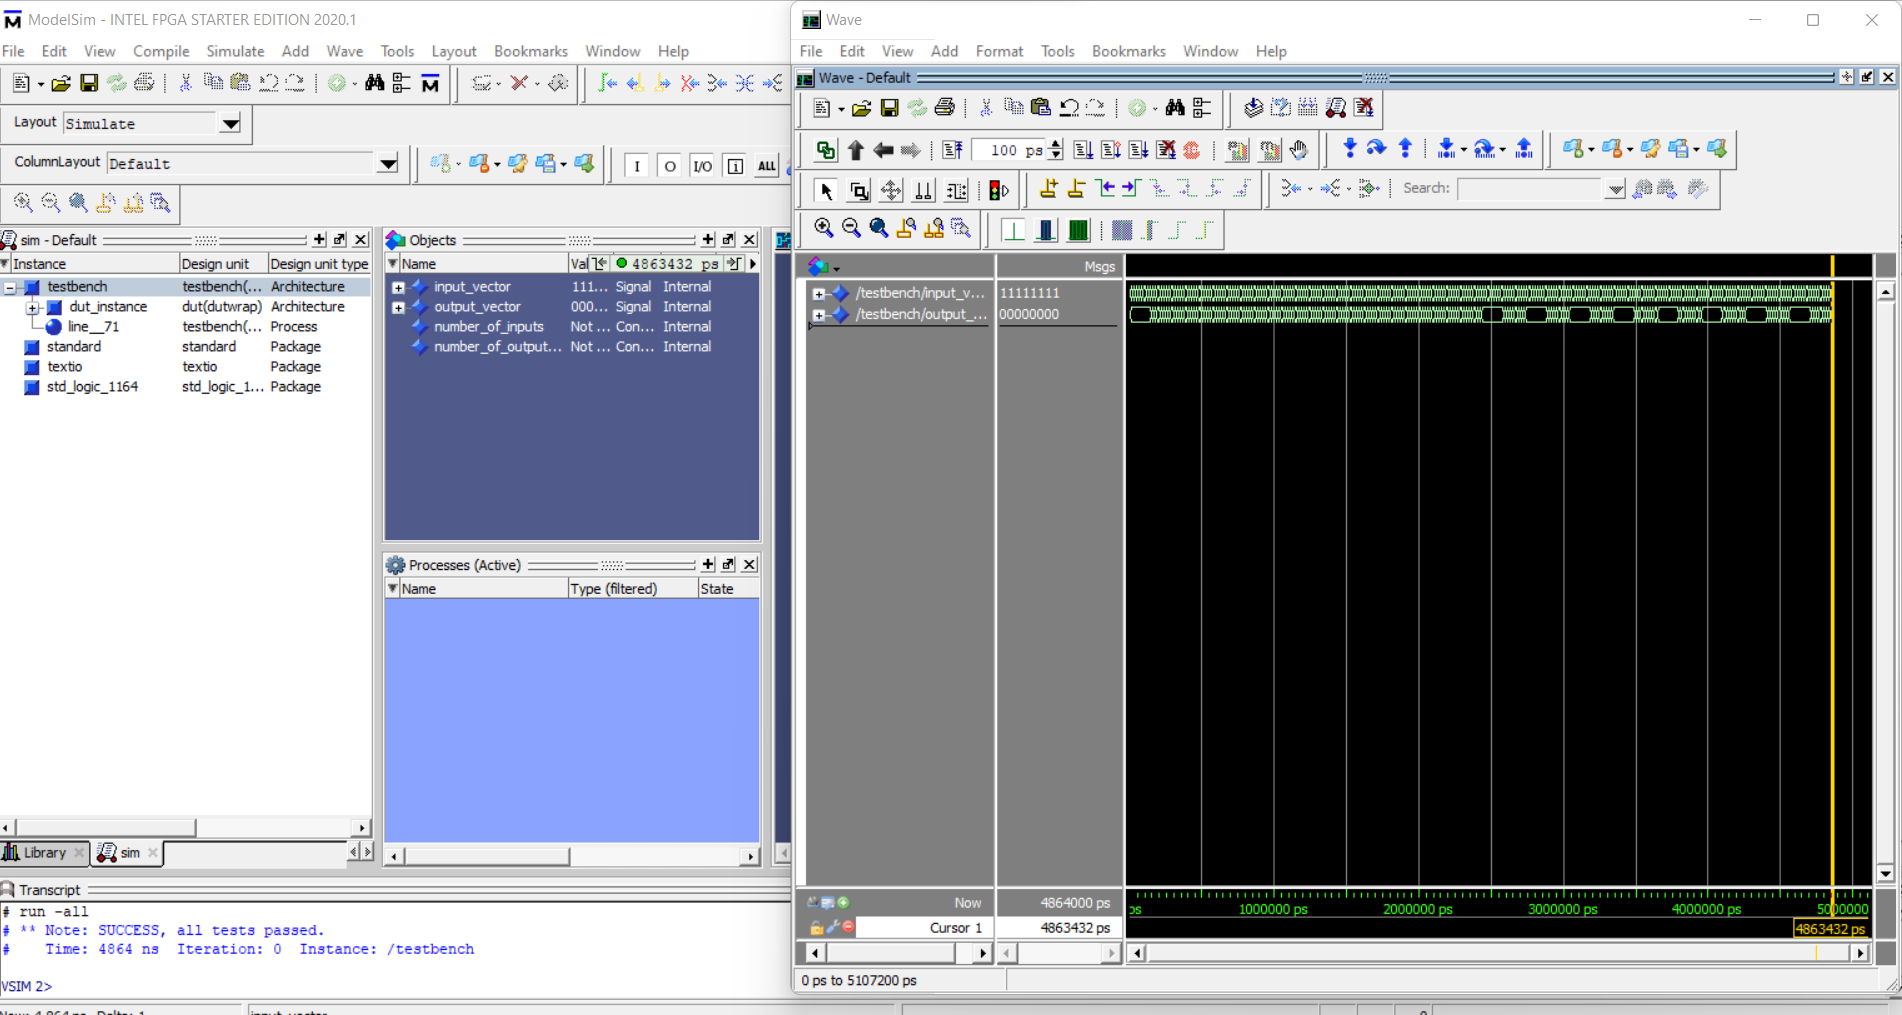
\includegraphics[scale=0.35]{Images/ALU_RTLSimulation.png}
  \caption{ALU RTL Simulation Waveform}
\end{figure}

Further the code (in form of .svf file) was flashed onto the Xen10 board. Then scanchain was run to generate outputs using tracefile and then compared to the golden outputs to check if the outputs were indeed correct. The output was verified, which also verified the working of the logic for the ALU. The output file's content is shown below.

\begin{verbatim}
00000000 00000000 Success
00000001 00000000 Success
00000010 00000000 Success
00000011 00000000 Success
00000100 00000000 Success
00000101 00000000 Success
00000110 00000000 Success
00000111 00000000 Success
00001000 00001000 Success
00001001 00001001 Success
00001010 00001010 Success
00001011 00001011 Success
00001100 00001100 Success
00001101 00001101 Success
00001110 00001110 Success
00001111 00001111 Success
00010000 00000001 Success
00010001 00000010 Success
00010010 00000100 Success
00010011 00001000 Success
00010100 00010000 Success
00010101 00100000 Success
00010110 01000000 Success
00010111 10000000 Success
00011000 00000111 Success
00011001 00001000 Success
00011010 00001001 Success
00011011 00001010 Success
00011100 00001011 Success
00011101 00001100 Success
00011110 00001101 Success
00011111 00001110 Success
00100000 00000010 Success
00100001 00000100 Success
00100010 00001000 Success
00100011 00010000 Success
00100100 00100000 Success
00100101 01000000 Success
00100110 10000000 Success
00100111 00000001 Success
00101000 00000110 Success
00101001 00000111 Success
00101010 00001000 Success
00101011 00001001 Success
00101100 00001010 Success
00101101 00001011 Success
00101110 00001100 Success
00101111 00001101 Success
00110000 00000011 Success
00110001 00000110 Success
00110010 00001100 Success
00110011 00011000 Success
00110100 00110000 Success
00110101 01100000 Success
00110110 11000000 Success
00110111 10000001 Success
00111000 00000101 Success
00111001 00000110 Success
00111010 00000111 Success
00111011 00001000 Success
00111100 00001001 Success
00111101 00001010 Success
00111110 00001011 Success
00111111 00001100 Success
01000000 00000100 Success
01000001 00001000 Success
01000010 00010000 Success
01000011 00100000 Success
01000100 01000000 Success
01000101 10000000 Success
01000110 00000001 Success
01000111 00000010 Success
01001000 00000100 Success
01001001 00000101 Success
01001010 00000110 Success
01001011 00000111 Success
01001100 00001000 Success
01001101 00001001 Success
01001110 00001010 Success
01001111 00001011 Success
01010000 00000101 Success
01010001 00001010 Success
01010010 00010100 Success
01010011 00101000 Success
01010100 01010000 Success
01010101 10100000 Success
01010110 01000001 Success
01010111 10000010 Success
01011000 00000011 Success
01011001 00000100 Success
01011010 00000101 Success
01011011 00000110 Success
01011100 00000111 Success
01011101 00001000 Success
01011110 00001001 Success
01011111 00001010 Success
01100000 00000110 Success
01100001 00001100 Success
01100010 00011000 Success
01100011 00110000 Success
01100100 01100000 Success
01100101 11000000 Success
01100110 10000001 Success
01100111 00000011 Success
01101000 00000010 Success
01101001 00000011 Success
01101010 00000100 Success
01101011 00000101 Success
01101100 00000110 Success
01101101 00000111 Success
01101110 00001000 Success
01101111 00001001 Success
01110000 00000111 Success
01110001 00001110 Success
01110010 00011100 Success
01110011 00111000 Success
01110100 01110000 Success
01110101 11100000 Success
01110110 11000001 Success
01110111 10000011 Success
01111000 00000001 Success
01111001 00000010 Success
01111010 00000011 Success
01111011 00000100 Success
01111100 00000101 Success
01111101 00000110 Success
01111110 00000111 Success
01111111 00001000 Success
10000000 00101000 Success
10000001 00101000 Success
10000010 00101000 Success
10000011 00101000 Success
10000100 00101000 Success
10000101 00101000 Success
10000110 00101000 Success
10000111 00101000 Success
10001000 00000000 Success
10001001 00000001 Success
10001010 00000010 Success
10001011 00000011 Success
10001100 00000100 Success
10001101 00000101 Success
10001110 00000110 Success
10001111 00000111 Success
10010000 00101101 Success
10010001 00101101 Success
10010010 00101101 Success
10010011 00101101 Success
10010100 00101101 Success
10010101 00101101 Success
10010110 00101101 Success
10010111 00101101 Success
10011000 00000001 Success
10011001 00000000 Success
10011010 00000011 Success
10011011 00000010 Success
10011100 00000101 Success
10011101 00000100 Success
10011110 00000111 Success
10011111 00000110 Success
10100000 00110010 Success
10100001 00110010 Success
10100010 00110010 Success
10100011 00110010 Success
10100100 00110010 Success
10100101 00110010 Success
10100110 00110010 Success
10100111 00110010 Success
10101000 00000010 Success
10101001 00000011 Success
10101010 00000000 Success
10101011 00000001 Success
10101100 00000110 Success
10101101 00000111 Success
10101110 00000100 Success
10101111 00000101 Success
10110000 00110111 Success
10110001 00110111 Success
10110010 00110111 Success
10110011 00110111 Success
10110100 00110111 Success
10110101 00110111 Success
10110110 00110111 Success
10110111 00110111 Success
10111000 00000011 Success
10111001 00000010 Success
10111010 00000001 Success
10111011 00000000 Success
10111100 00000111 Success
10111101 00000110 Success
10111110 00000101 Success
10111111 00000100 Success
11000000 00111100 Success
11000001 00111100 Success
11000010 00111100 Success
11000011 00111100 Success
11000100 00111100 Success
11000101 00111100 Success
11000110 00111100 Success
11000111 00111100 Success
11001000 00000100 Success
11001001 00000101 Success
11001010 00000110 Success
11001011 00000111 Success
11001100 00000000 Success
11001101 00000001 Success
11001110 00000010 Success
11001111 00000011 Success
11010000 01000001 Success
11010001 01000001 Success
11010010 01000001 Success
11010011 01000001 Success
11010100 01000001 Success
11010101 01000001 Success
11010110 01000001 Success
11010111 01000001 Success
11011000 00000101 Success
11011001 00000100 Success
11011010 00000111 Success
11011011 00000110 Success
11011100 00000001 Success
11011101 00000000 Success
11011110 00000011 Success
11011111 00000010 Success
11100000 01000110 Success
11100001 01000110 Success
11100010 01000110 Success
11100011 01000110 Success
11100100 01000110 Success
11100101 01000110 Success
11100110 01000110 Success
11100111 01000110 Success
11101000 00000110 Success
11101001 00000111 Success
11101010 00000100 Success
11101011 00000101 Success
11101100 00000010 Success
11101101 00000011 Success
11101110 00000000 Success
11101111 00000001 Success
11110000 01001011 Success
11110001 01001011 Success
11110010 01001011 Success
11110011 01001011 Success
11110100 01001011 Success
11110101 01001011 Success
11110110 01001011 Success
11110111 01001011 Success
11111000 00000111 Success
11111001 00000110 Success
11111010 00000101 Success
11111011 00000100 Success
11111100 00000011 Success
11111101 00000010 Success
11111110 00000001 Success
11111111 00000000 Success
\end{verbatim}

\end{document}